elli fyllir út, TODO
\subsubsection{upprunalega/inngangur/greining}
lýsing á vélbúnaðinum og greiningu á virkni hans.. \\\\
\begin{figure}[H]
    \centering
    \begin{tikzpicture}[
        node distance=3cm,    % Distance between the nodes
        auto,                 % Automatically adjust positioning of labels
        >=latex,              % Arrow style
        every node/.style={draw, rectangle, minimum height=1.2cm, minimum width=2.5cm, align=center}
    ]
    % Define the nodes with text inside boxes
    \node (q0) {Ljósskynjari};
    \node (q1) [right of=q0] {Sleði};
    \node (q2) [right of=q1] {Console};
    
    % Draw arrows between the boxes
    \draw[->] (q0) -- (q1);
    \draw[->] (q1) -- (q2);
    
    \end{tikzpicture}
    \caption{Caption}
    \label{fig:enter-label}
\end{figure}

\subsubsection{hugmynd að útfærslu}
fjallað um breytingar


\begin{figure}
    \centering
    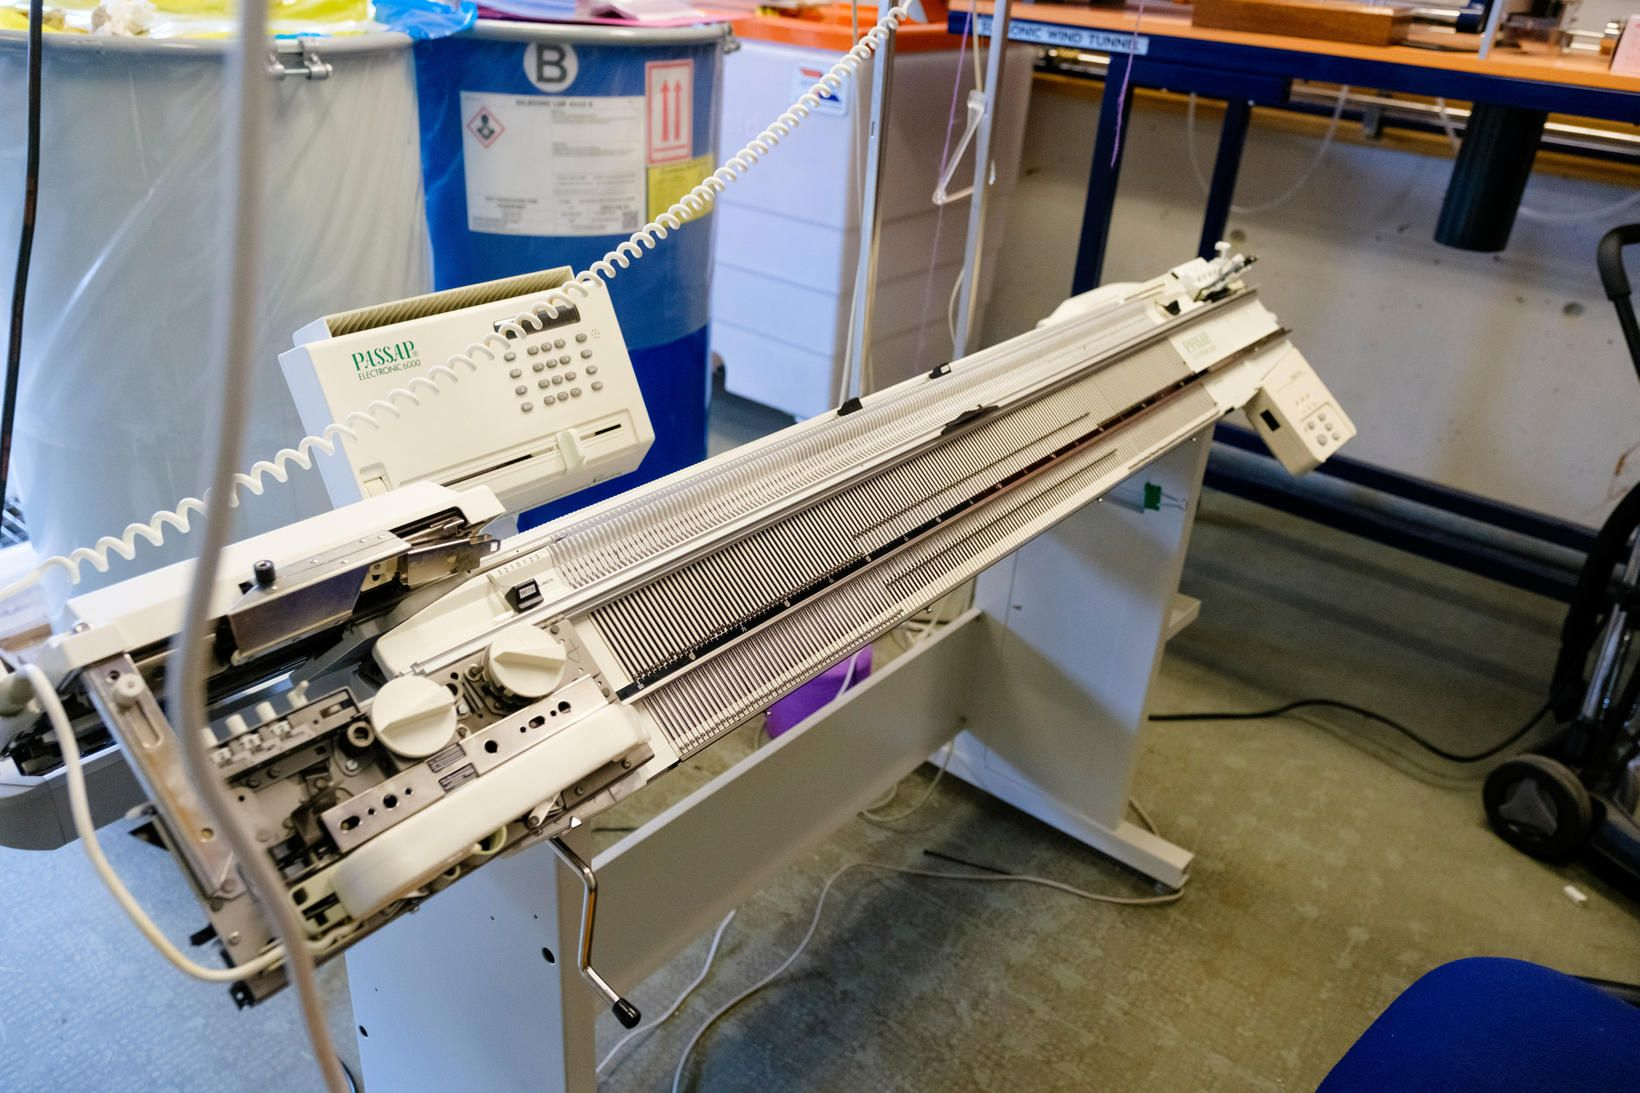
\includegraphics[width=0.5\linewidth]{myndir/elli/e6000.jpg}
    \caption{\textit{Passap E6000} prjónavél - \textit{mbl.is/Kristinn Magnússon}}
    \label{fig:e6000}
\end{figure}

\begin{figure}
    \centering
    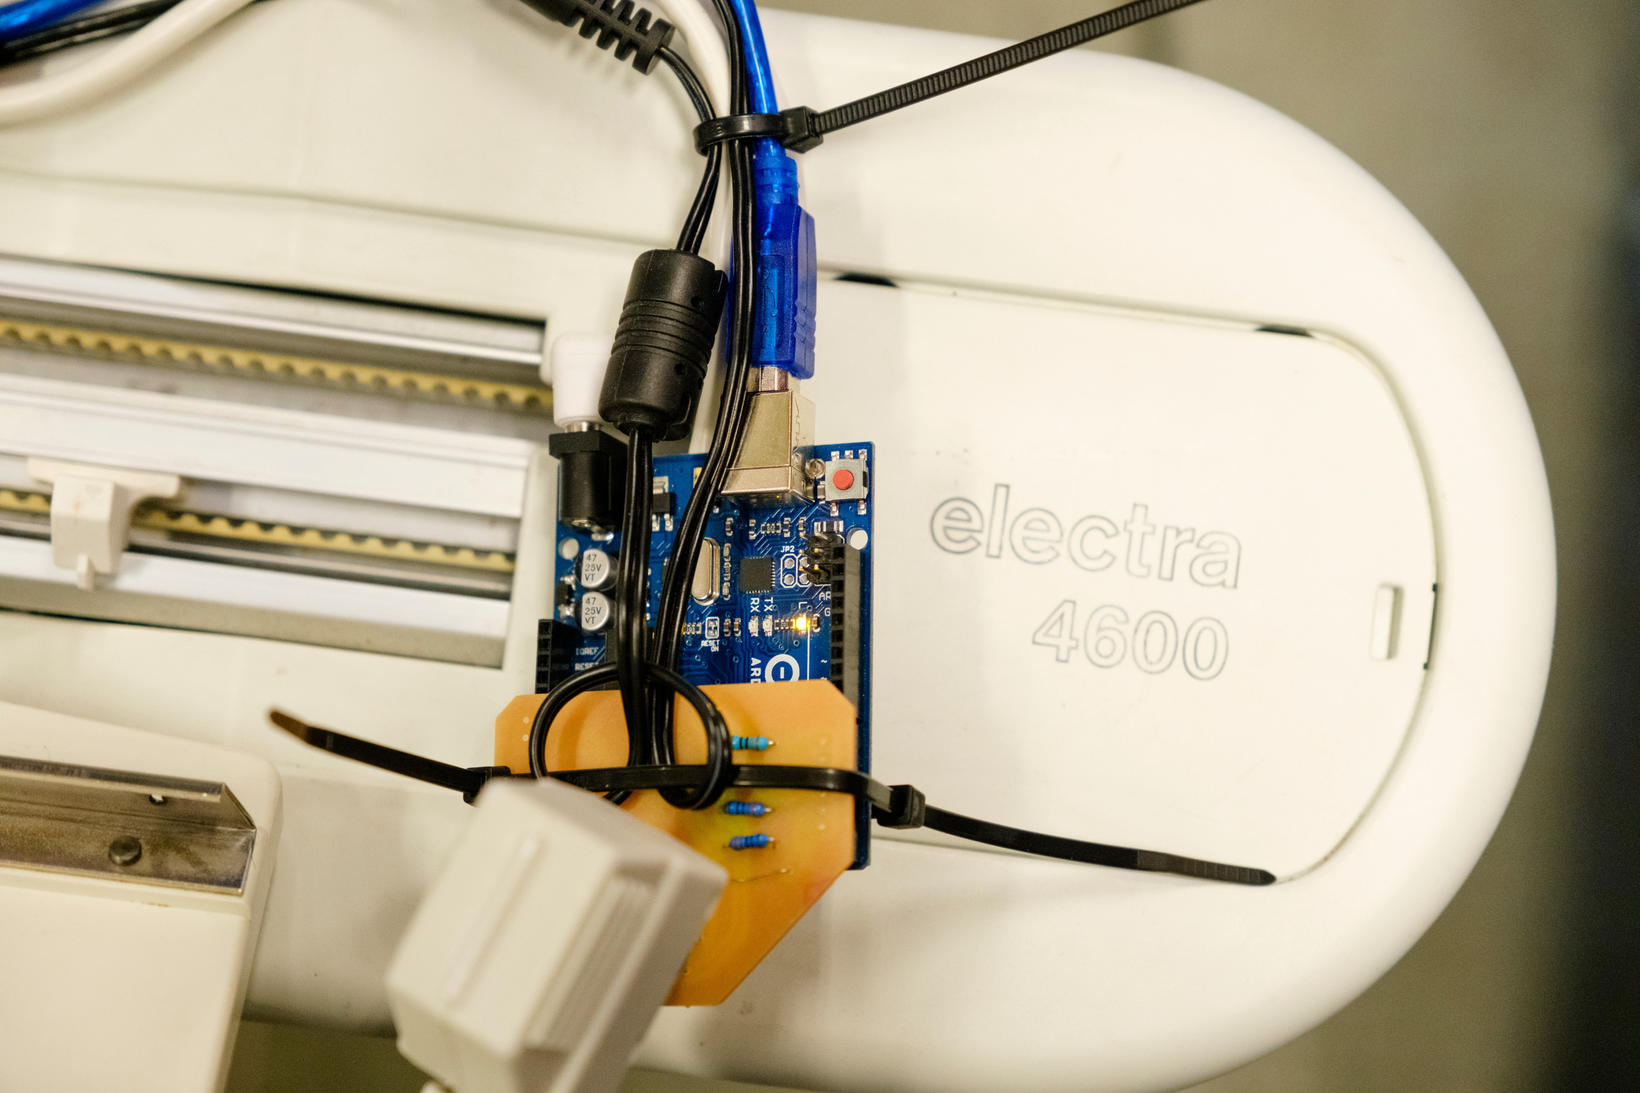
\includegraphics[width=0.5\linewidth]{myndir/elli/electra4600.jpg}
    \caption{Arduino örtölva tengd við \textit{Passap E6000} - \textit{mbl.is/Kristinn Magnússon}}
    \label{fig:arduino}
\end{figure}